% Options for packages loaded elsewhere
% Options for packages loaded elsewhere
\PassOptionsToPackage{unicode}{hyperref}
\PassOptionsToPackage{hyphens}{url}
\PassOptionsToPackage{dvipsnames,svgnames,x11names}{xcolor}
%
\documentclass[
  12pt]{article}
\usepackage{xcolor}
\usepackage{amsmath,amssymb}
\setcounter{secnumdepth}{5}
\usepackage{iftex}
\ifPDFTeX
  \usepackage[T1]{fontenc}
  \usepackage[utf8]{inputenc}
  \usepackage{textcomp} % provide euro and other symbols
\else % if luatex or xetex
  \usepackage{unicode-math} % this also loads fontspec
  \defaultfontfeatures{Scale=MatchLowercase}
  \defaultfontfeatures[\rmfamily]{Ligatures=TeX,Scale=1}
\fi
\usepackage{lmodern}
\ifPDFTeX\else
  % xetex/luatex font selection
\fi
% Use upquote if available, for straight quotes in verbatim environments
\IfFileExists{upquote.sty}{\usepackage{upquote}}{}
\IfFileExists{microtype.sty}{% use microtype if available
  \usepackage[]{microtype}
  \UseMicrotypeSet[protrusion]{basicmath} % disable protrusion for tt fonts
}{}
\makeatletter
\@ifundefined{KOMAClassName}{% if non-KOMA class
  \IfFileExists{parskip.sty}{%
    \usepackage{parskip}
  }{% else
    \setlength{\parindent}{0pt}
    \setlength{\parskip}{6pt plus 2pt minus 1pt}}
}{% if KOMA class
  \KOMAoptions{parskip=half}}
\makeatother
% Make \paragraph and \subparagraph free-standing
\makeatletter
\ifx\paragraph\undefined\else
  \let\oldparagraph\paragraph
  \renewcommand{\paragraph}{
    \@ifstar
      \xxxParagraphStar
      \xxxParagraphNoStar
  }
  \newcommand{\xxxParagraphStar}[1]{\oldparagraph*{#1}\mbox{}}
  \newcommand{\xxxParagraphNoStar}[1]{\oldparagraph{#1}\mbox{}}
\fi
\ifx\subparagraph\undefined\else
  \let\oldsubparagraph\subparagraph
  \renewcommand{\subparagraph}{
    \@ifstar
      \xxxSubParagraphStar
      \xxxSubParagraphNoStar
  }
  \newcommand{\xxxSubParagraphStar}[1]{\oldsubparagraph*{#1}\mbox{}}
  \newcommand{\xxxSubParagraphNoStar}[1]{\oldsubparagraph{#1}\mbox{}}
\fi
\makeatother


\usepackage{longtable,booktabs,array}
\newcounter{none} % for unnumbered tables
\usepackage{calc} % for calculating minipage widths
% Correct order of tables after \paragraph or \subparagraph
\usepackage{etoolbox}
\makeatletter
\patchcmd\longtable{\par}{\if@noskipsec\mbox{}\fi\par}{}{}
\makeatother
% Allow footnotes in longtable head/foot
\IfFileExists{footnotehyper.sty}{\usepackage{footnotehyper}}{\usepackage{footnote}}
\makesavenoteenv{longtable}
\usepackage{graphicx}
\makeatletter
\newsavebox\pandoc@box
\newcommand*\pandocbounded[1]{% scales image to fit in text height/width
  \sbox\pandoc@box{#1}%
  \Gscale@div\@tempa{\textheight}{\dimexpr\ht\pandoc@box+\dp\pandoc@box\relax}%
  \Gscale@div\@tempb{\linewidth}{\wd\pandoc@box}%
  \ifdim\@tempb\p@<\@tempa\p@\let\@tempa\@tempb\fi% select the smaller of both
  \ifdim\@tempa\p@<\p@\scalebox{\@tempa}{\usebox\pandoc@box}%
  \else\usebox{\pandoc@box}%
  \fi%
}
% Set default figure placement to htbp
\def\fps@figure{htbp}
\makeatother





\setlength{\emergencystretch}{3em} % prevent overfull lines

\providecommand{\tightlist}{%
  \setlength{\itemsep}{0pt}\setlength{\parskip}{0pt}}



 
\usepackage[]{natbib}
\bibliographystyle{agsm}


\addtolength{\oddsidemargin}{-.5in}%
\addtolength{\evensidemargin}{-1in}%
\addtolength{\textwidth}{1in}%
\addtolength{\textheight}{1.7in}%
\addtolength{\topmargin}{-1in}%
% agsm.bst prints URLs with \harvardurl, which natbib typesets as
% plain italic text; that breaks on URLs with underscores, so use \url
\AtBeginDocument{\def\harvardurl{\url}}
\makeatletter
\@ifpackageloaded{caption}{}{\usepackage{caption}}
\AtBeginDocument{%
\ifdefined\contentsname
  \renewcommand*\contentsname{Table of contents}
\else
  \newcommand\contentsname{Table of contents}
\fi
\ifdefined\listfigurename
  \renewcommand*\listfigurename{List of Figures}
\else
  \newcommand\listfigurename{List of Figures}
\fi
\ifdefined\listtablename
  \renewcommand*\listtablename{List of Tables}
\else
  \newcommand\listtablename{List of Tables}
\fi
\ifdefined\figurename
  \renewcommand*\figurename{Figure}
\else
  \newcommand\figurename{Figure}
\fi
\ifdefined\tablename
  \renewcommand*\tablename{Table}
\else
  \newcommand\tablename{Table}
\fi
}
\@ifpackageloaded{float}{}{\usepackage{float}}
\floatstyle{ruled}
\@ifundefined{c@chapter}{\newfloat{codelisting}{h}{lop}}{\newfloat{codelisting}{h}{lop}[chapter]}
\floatname{codelisting}{Listing}
\newcommand*\listoflistings{\listof{codelisting}{List of Listings}}
\makeatother
\makeatletter
\makeatother
\makeatletter
\@ifpackageloaded{caption}{}{\usepackage{caption}}
\@ifpackageloaded{subcaption}{}{\usepackage{subcaption}}
\makeatother
\usepackage{bookmark}
\IfFileExists{xurl.sty}{\usepackage{xurl}}{} % add URL line breaks if available
\urlstyle{same}
% fallback for those not using the hyperref driver hyperxmp:
\makeatletter
\@ifundefined{xmpquote}{\newcommand{\xmpquote}[1]{#1}}{}
\makeatother
\hypersetup{
  pdftitle={Prior Ridge: Regularization for FRC Rating},
  pdfauthor={Gabriel Krotkov; Mitchell G. Hung; Rosy Yu},
  pdfkeywords={\xmpquote{ridge
regression}, \xmpquote{regularization}, \xmpquote{rating
systems}, \xmpquote{Elo ratings}, \xmpquote{FIRST Robotics
Competition}},
  colorlinks=true,
  linkcolor={blue},
  filecolor={Maroon},
  citecolor={Blue},
  urlcolor={Blue},
  pdfcreator={LaTeX via pandoc}}



\begin{document}


\def\spacingset#1{\renewcommand{\baselinestretch}%
{#1}\small\normalsize} \spacingset{1}


%%%%%%%%%%%%%%%%%%%%%%%%%%%%%%%%%%%%%%%%%%%%%%%%%%%%%%%%%%%%%%%%%%%%%%%%%%%%%%

\date{October 4, 2026}
\title{\bf Prior Ridge: Regularization for FRC Rating}
\author{
Gabriel Krotkov\\
Mentor, FRC 449 \& 4821\\
and\\Mitchell G. Hung\\
Data Science Lead, FRC 449\\
and\\Rosy Yu\\
Data Science, FRC 449\\
}
\maketitle

\bigskip
\bigskip
\begin{abstract}
In FRC (the FIRST Robotics Competition), there are two primary team
rating models: OPR (Offensive Power Rating) and EPA (Expected Points
Added). OPR is statistically efficient and unbiased, but has no memory
between events and is essentially starting from scratch every event.
Starting fresh every event means that OPR tends to have high variance,
and often doesn't have enough data to stabilize. EPA achieves better
prediction by incorporating historical information, but trades off
statistical efficiency to do so---EPA doesn't learn from new data as
fast as OPR. Prior Ridge (pRidge) applies Bayesian-inspired
regularization to balance between the relatively high variance of OPR
and the relatively high bias of EPA. On average over all qualifier
events between 2016 and 2026, Prior Ridge overperforms OPR by 15.4\% in
terms of cross validated mean squared error, and overperforms EPA by
11.1\% in terms of next-match-prediction error.
\end{abstract}

\noindent%
{\it Keywords:} ridge regression, regularization, rating systems, Elo
ratings, FIRST Robotics Competition
\vfill

\newpage
\spacingset{1.9} % DON'T change the spacing!


\section{Introduction}\label{introduction}

\subsection{Motivation: the bias-variance
tradeoff}\label{motivation-the-bias-variance-tradeoff}

The two primary models for team rating in FRC neatly illustrate a
bias-variance tradeoff common in real-world modeling. OPR\footnote{We
  will refer to linear regression in an FRC context as OPR for
  familiarity, although other names outlined in Table~\ref{tbl-methods}
  may be more descriptive.} is a special case of linear regression,
which is provably a minimum variance linear unbiased estimator. That is,
if you require unbiasedness and agree with the linear regression
assumptions, OPR is provably optimal \citep{gauss_markov}. However, you
can often improve an estimator's prediction by accepting some bias to
reduce variance. Statbotics' EPA \citep{statbotics_eval} does exactly
this. By incorporating information about teams' historical performance,
EPA accepts statistical bias in exchange for much faster convergence.
This is a good fit for the FRC setting, where teams rarely have more
than 12 qualification matches at an event (and often have fewer), so
data is relatively scarce.

This leaves considerable room for optimization. Exactly how much prior
information to incorporate is a hard challenge to resolve. Luckily,
there's an established body of regularization tools from regression
analysis aimed specifically at solving this problem\footnote{In fact, in
  NBA sports analytics (a similar data setting to FRC), RAPM
  \citep{rapm_cmu} is an example of using regularization to improve on
  ordinary least squares regression popular since at least 2017
  \citep{rapm_blog}.}. Prior Ridge (pRidge) applies those tools with a
Bayesian twist to optimize the bias-variance tradeoff between OPR and
EPA and pick more predictive coefficients.

\subsection{Background}\label{background}

At FRC events, teams play matches in 3-team ``alliances'' with shared
results. Like in any team sport, shared results pose a challenge for
rating systems---it's hard to parse out individual team performance from
alliance--level results. Taking a team's average alliance score and
dividing by 3 is a reasonable first guess at their offensive
contribution---but the FRC community has developed better methods for
team rating.

\subsubsection{FRC Linear Regression
(OPR)}\label{frc-linear-regression-opr}

One influential rating method is OPR (``Offensive Power Rating''),
described in Eugene Fang's The Blue Alliance blog \citep{opr_blog}. OPR
is a special case of multiple linear regression with a zero intercept.
We set it up as a system of equations where each team's contribution is
a variable, and each alliance's performance is represented as an
equation (ex. \(red1 + red2 + red3 = redScore\)). Each match generates
two equations, one for the red alliance, and one for the blue alliance.
OPR is then just the least-squares approximate solution to this system.
This is identical to the way linear regression minimizes the squared
error between predicted and actual values. More formally, the OPR
equation \(Mx = s\) consists of \(M\) (a matrix with alliances as rows
and teams as columns), \(x\) (the vector of team coefficients we solve
for), and \(s\) (the observed alliance scores). This mirrors the
standard linear regression formulation \(y = X\beta\)
\citep[sec.~3.2]{ISLR}, which solves for coefficients \(\beta\) by
minimizing squared residuals.

\subsubsection{FRC Elo ratings (Statbotics
EPA)}\label{frc-elo-ratings-statbotics-epa}

Statbotics' EPA (``Expected Points Added'') is another popular FRC
rating method. EPA \citep{epa_intro} is adapted from the Elo rating
system, initially designed for 1v1 Chess for 3v3 FRC. Unitless EPA, a
metric very similar to Elo in its non-specificity to a certain season's
game, takes into account previous season performance for a first
estimate. To produce the version of EPA used for score predictions,
unitless EPA scales by the standard deviation of Week 1 scores,
effectively adopting the ``units'' of a particular year's points system.
EPA updates are adjusted based on the ``shock of victory'', modeled by
\(K\) and \(M\). \(K\) is the learning rate for EPA: a higher \(K\)
means that EPA adjusts more based on the result of each match. \(M\) is
the margin parameter, which defines how much the EPA update cares about
the opposing alliance's performance. Both \(M\) and \(K\) are defined
piecewise in terms of the number of matches played, with \(M\)
increasing and \(K\) decreasing as the season continues. Unlike
traditional Elo, EPA is designed to be a non-zero sum model: when one
team's EPA increases, others don't necessarily decrease, which can
reflect increasing team performance over the season.

\begin{longtable}[]{@{}
  >{\raggedright\arraybackslash}p{(\linewidth - 4\tabcolsep) * \real{0.2436}}
  >{\raggedright\arraybackslash}p{(\linewidth - 4\tabcolsep) * \real{0.3846}}
  >{\raggedright\arraybackslash}p{(\linewidth - 4\tabcolsep) * \real{0.3718}}@{}}
\caption{Mapping FRC rating systems onto statistical
methods}\label{tbl-methods}\tabularnewline
\toprule\noalign{}
\begin{minipage}[b]{\linewidth}\raggedright
Method
\end{minipage} & \begin{minipage}[b]{\linewidth}\raggedright
FRC Domain Name
\end{minipage} & \begin{minipage}[b]{\linewidth}\raggedright
Reference Implementations
\end{minipage} \\
\midrule\noalign{}
\endfirsthead
\toprule\noalign{}
\begin{minipage}[b]{\linewidth}\raggedright
Method
\end{minipage} & \begin{minipage}[b]{\linewidth}\raggedright
FRC Domain Name
\end{minipage} & \begin{minipage}[b]{\linewidth}\raggedright
Reference Implementations
\end{minipage} \\
\midrule\noalign{}
\endhead
\bottomrule\noalign{}
\endlastfoot
Linear Regression & OPR, Calculated Contribution & TheBlueAlliance
Insights \\
Elo Ratings & EPA & Statbotics, Caleb Sykes Elo \\
\end{longtable}

\subsubsection{Overfitting and
Regularization}\label{overfitting-and-regularization}

Overfitting is a typical modeling issue that comes from fitting your
training data too closely, usually because of high model complexity. In
Figure~\ref{fig-overfitting}, the blue dots represent training data, and
the red and green curves are candidate models to fit the data. The red
curve represents a complicated, high degree polynomial fit, while the
green line represents a simple linear fit. The training error of the red
line is exactly zero, since the model exactly intersects each dot, while
the green model has some error due to random variance. Even though the
red model has a lower training error than the green model, if we were to
test against data outside this sample, the simpler green model is almost
sure to perform better. We call the red model in this case ``overfit'' -
that is, matching the training dataset too closely.

Regularization \citep[sec.~6.2.1]{ISLR} is the process of correcting for
overfitting to improve the generalizability of a model. A common way to
do this is by adding a penalty for complexity to the model. This forces
the model optimization to weigh the cost of additional complexity
against the performance gain on the training data. This can
significantly improve a model's generalizability, especially when the
exact value of the penalty is carefully chosen.

\begin{figure}[htbp]

\centering{

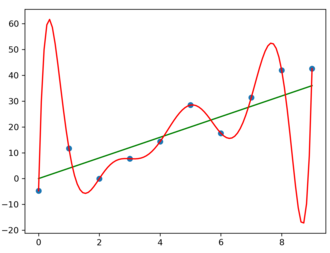
\includegraphics[width=0.4\linewidth,height=\textheight,keepaspectratio]{images/overfitting_wikipedia.png}

}

\caption{\label{fig-overfitting}Overfitting example. Image:
\href{https://commons.wikimedia.org/wiki/File:Pyplot_overfitting.png}{``Pyplot
overfitting''} by ThirdOrderLogic, via Wikimedia Commons, licensed under
\href{https://creativecommons.org/licenses/by/4.0/}{CC BY 4.0}.}

\end{figure}%

\section{Methods}\label{methods}

\subsection{Prior Ridge Model}\label{prior-ridge-model}

The Prior Ridge model is based on Ridge Regression
\citep[sec.~6.2.1]{ISLR}, which is a regularized version of ordinary
least squares regression. The loss function for ridge regression
includes a penalty term scaled by \(\lambda\), the regularization
parameter, which pushes all the coefficients in the model fit towards
zero by penalizing large coefficients. This introduces some bias
(towards zero), in exchange for considerably reducing estimate variance.
In many model settings, this is a good tradeoff, and the simpler
regularized model generalizes better than the optimal fit on training
data. However, we can do better than regularizing towards zero. If we
have an informative prior - that is, a good guess going into the event
about the team's rating - we can instead regularize towards \emph{that}
by penalizing the distance from the priors rather than penalizing the
magnitude of the coefficients (derivation in
Section~\ref{sec-derivation}). Statbotics EPA provides us with exactly
that - a very good guess as to the team's actual per-match contribution.
Prior Ridge is essentially OPR, with a trick layered on top: regularize
towards pre-event Statbotics EPA as a prior. While the fundamental model
still works with other priors (for example, season max OPR), we chose
Statbotics EPA for familiarity and to explicitly optimize the balance
between major rating methods.

\[
\begin{aligned}
\text{OLS:} \quad \hat{\beta} &= (X^TX)^{-1}(X^Ty) \\
\text{Ridge:} \quad \hat{\beta} &= (X^TX + \lambda I)^{-1}(X^Ty) \\
\text{pRidge:} \quad \hat{\beta} &= (X^TX + \lambda I)^{-1}(X^Ty + \lambda \beta_0)
\end{aligned}
\]

\subsection{\texorpdfstring{Picking
\(\lambda\)}{Picking \textbackslash lambda}}\label{picking-lambda}

Picking a good value of \(\lambda\) is the core challenge to making
pRidge effective. \(\lambda\) controls bias-variance balance
\citep[sec.~2.2.2]{ISLR} between the priors and new data. On one hand,
pRidge with \(\lambda = 0\) is simply equivalent to OPR. On the other,
pRidge with \(\lambda = \infty\) makes predictions solely based on the
EPA priors without any update. To optimize the choice of \(\lambda\), we
use leave-one-out cross validation (LOOCV) \citep[pp.~200--203]{ISLR} to
evaluate a grid of \(\lambda\) choices and select the one with minimal
LOOCV mean squared error (MSE). \(\lambda\) is re-optimized with each
new fit of the pRidge model to data.

We chose a \(\lambda\) grid of all values between 0.01 and 20 evenly
spaced on a log scale. Keeping the lower limit above 0 guarantees that
the matrix is positive-definite, while 20 is an arbitrarily chosen upper
bound based on exploratory cross validation plots (for an example,
Figure~\ref{fig-severn-cv}). Searching the grid on a log scale instead
of a linear scale helps preserve computational effort by allocating
precision to the more useful part of the range. For instance, the
difference between \(\lambda = 16.2\) and \(\lambda = 16\) is much less
meaningful than the difference between \(\lambda = 1.2\) and
\(\lambda = 1\).

\begin{figure}[htbp]

\begin{minipage}[t]{0.50\linewidth}

\centering{

\pandocbounded{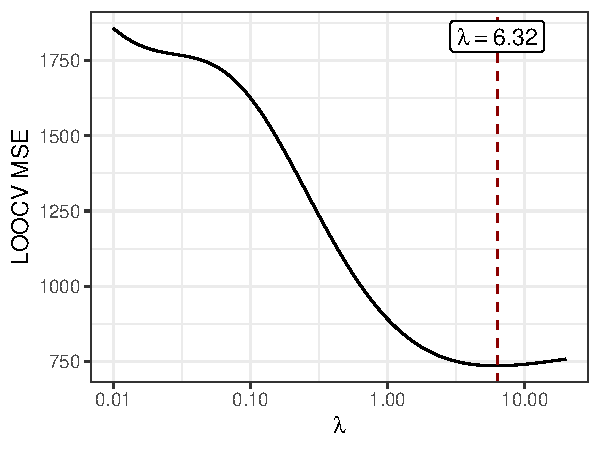
\includegraphics[keepaspectratio]{index_files/figure-pdf/fig-severn-qm16-1.pdf}}

}

\subcaption{\label{fig-severn-qm16}With 16 matches complete}

\end{minipage}%
%
\begin{minipage}[t]{0.50\linewidth}

\centering{

\pandocbounded{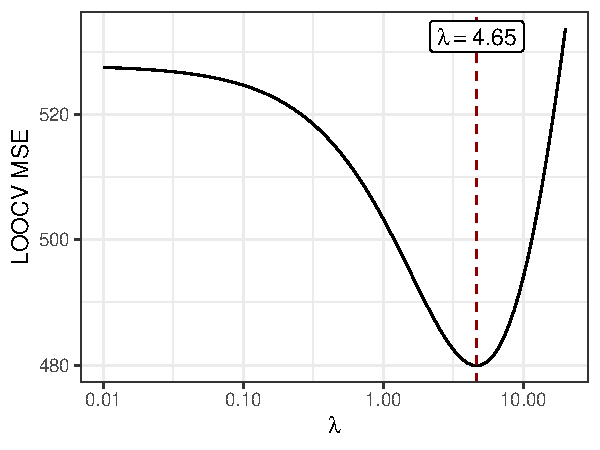
\includegraphics[keepaspectratio]{index_files/figure-pdf/fig-severn-full-1.pdf}}

}

\subcaption{\label{fig-severn-full}With all matches complete}

\end{minipage}%

\caption{\label{fig-severn-cv}pRidge Cross Validation for 2025 Severn
District}

\end{figure}%

\subsection{Cross validation evaluation against
OPR}\label{cross-validation-evaluation-against-opr}

Both pRidge and OPR are fundamentally regression models, which makes
comparing their performance easier. To evaluate the performance of
pRidge against OPR, we used 4-fold cross validation on both models so
all matches were represented in the test set at least once for each
model, and then averaged the test MSE across folds. To preserve the
separation of \(\lambda\) selection and model evaluation, we nested the
LOOCV for \(\lambda\) selection inside the 4-fold cross validation for
model evaluation. This also drove the choice of \(k = 4\): this limited
the computational cost for nested cross validation loops.

\subsection{Next-match-prediction evaluation against
EPA}\label{next-match-prediction-evaluation-against-epa}

Selecting a fair comparison between pRidge and EPA is less direct,
because pRidge is order-invariant while EPA is order-dependent. To
evaluate between the models fairly, we designed a ``next-match
prediction'' procedure as follows. For each match at each event,
starting at the first match (i) for which OPR was valid to compute,
compute a prediction for match (i + 1) for both pRidge and EPA based
only on data up to match (i). Both models predict an alliance's score by
summing each team's rating value. This gives us a prediction for each
match after match (i) from which we can calculate an MSE for both
models.

\subsection{Estimating \% improvement}\label{estimating-improvement}

For both the OPR and EPA baseline evaluations, we computed the \%
improvement against the baseline as below, then took the mean across all
events and across years to estimate pRidge's improvement against
baseline models. We established the uncertainty in mean percent
improvements with a 95\% bootstrap \citep{uva_bootstrap} confidence
interval with 1 million replications.

\[
\%\ \text{improvement} = \frac{\text{MSE}_{\text{baseline}} - \text{MSE}_{\text{pRidge}}}{\text{MSE}_{\text{baseline}}}
\]

\subsection{Data}\label{data}

We used the TBA v3 API to access data from frc-events.firstinspires.org
to evaluate the performance of pRidge, EPA, and OPR. We chose to use
qualification matches from all regional and district qualifier events
between 2016 and 2026 (n = 1389), excepting events in 2020 and 2021 to
avoid seasons affected by the COVID-19 pandemic. We excluded playoff
matches since playoff alliances develop meaningfully different dynamics
than qualification matches with repeat partners and higher stakes. We
decided to start data collection in 2016 for API consistency and to
avoid Recycle Rush, a very atypical FRC game.

In our dataset, we were unable to compute a percent improvement for only
6 events when comparing to OPR, and only 6 events when comparing to EPA.
6 of these events in both cases were the 2026 Israel districts, 2022
Nanjing Regional, and the 2023 Izmir Regional, all of which were
canceled. The remaining fit failures overwhelmingly came from events
with 27 or fewer teams (ex. 2022mokc3, 2024vapor), typically in
pandemic-shortened 2022 events.

\section{Results}\label{results}

\begin{figure}[htbp]

\begin{minipage}[t]{0.50\linewidth}

\centering{

\pandocbounded{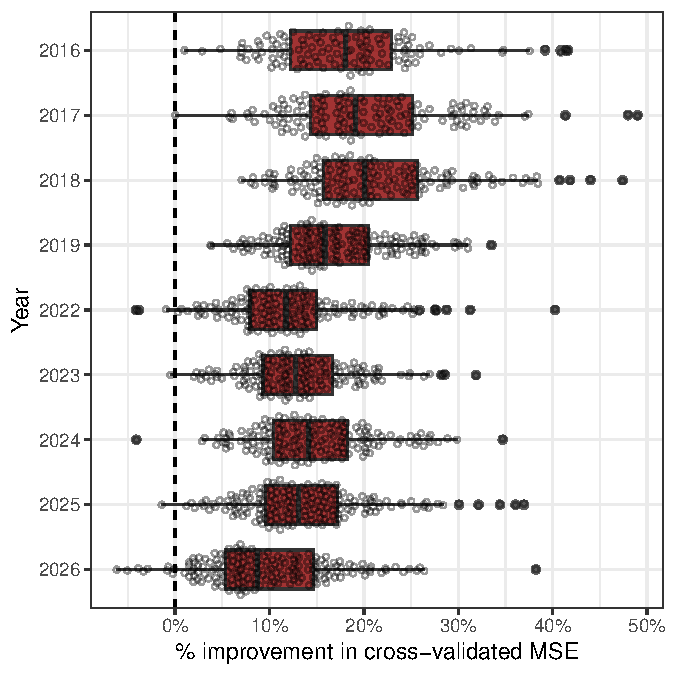
\includegraphics[keepaspectratio]{index_files/figure-pdf/fig-opr-year-1.pdf}}

}

\subcaption{\label{fig-opr-year}By year, OPR baseline}

\end{minipage}%
%
\begin{minipage}[t]{0.50\linewidth}

\centering{

\pandocbounded{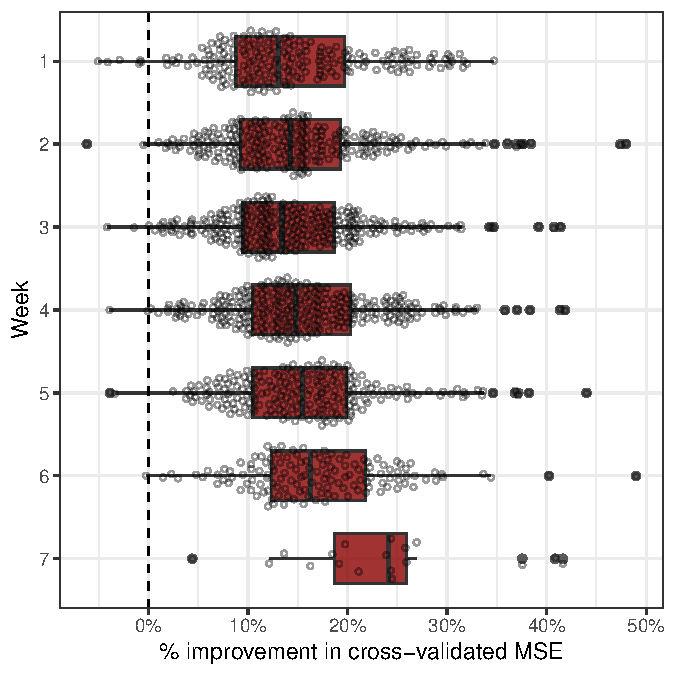
\includegraphics[keepaspectratio]{index_files/figure-pdf/fig-opr-week-1.pdf}}

}

\subcaption{\label{fig-opr-week}By week, OPR baseline}

\end{minipage}%
\newline
\begin{minipage}[t]{0.50\linewidth}

\centering{

\pandocbounded{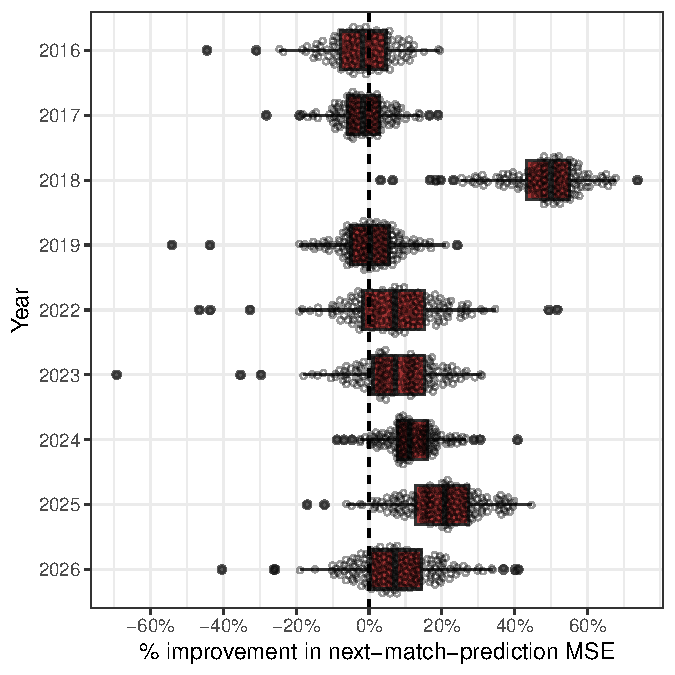
\includegraphics[keepaspectratio]{index_files/figure-pdf/fig-epa-year-1.pdf}}

}

\subcaption{\label{fig-epa-year}By year, EPA baseline}

\end{minipage}%
%
\begin{minipage}[t]{0.50\linewidth}

\centering{

\pandocbounded{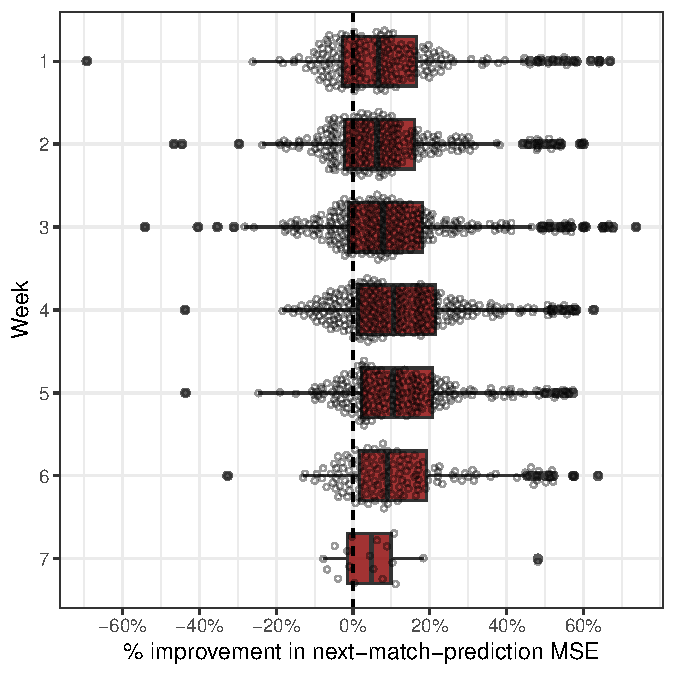
\includegraphics[keepaspectratio]{index_files/figure-pdf/fig-epa-week-1.pdf}}

}

\subcaption{\label{fig-epa-week}By week, EPA baseline}

\end{minipage}%

\caption{\label{fig-comparison}pRidge performance comparison against
baseline}

\end{figure}%

{

\begin{longtable}[]{@{}lrcc@{}}

\caption{\label{tbl-bootstrap}Bootstrap 95\% confidence intervals for
pRidge mean \% improvement, shown as (2.5th, 50th, 97.5th) percentiles}

\tabularnewline

\toprule\noalign{}
Year & \# Events & OPR Baseline & EPA Baseline \\
\midrule\noalign{}
\endhead
\bottomrule\noalign{}
\endlastfoot
Overall & 1389 & (15.0\%, 15.4\%, 15.8\%) & (10.2\%, 11.1\%, 12.1\%) \\
2016 & 118 & (16.9\%, 18.3\%, 19.7\%) & (−4.0\%, −2.2\%, −0.5\%) \\
2017 & 135 & (19.0\%, 20.4\%, 21.8\%) & (−2.7\%, −1.5\%, −0.2\%) \\
2018 & 148 & (20.1\%, 21.3\%, 22.6\%) & (45.9\%, 47.8\%, 49.6\%) \\
2019 & 162 & (16.0\%, 16.9\%, 17.9\%) & (−1.5\%, 0.0\%, 1.4\%) \\
2022 & 158 & (11.1\%, 12.1\%, 13.2\%) & (4.7\%, 6.9\%, 9.0\%) \\
2023 & 155 & (12.3\%, 13.2\%, 14.1\%) & (5.0\%, 7.0\%, 8.9\%) \\
2024 & 160 & (13.7\%, 14.7\%, 15.7\%) & (10.5\%, 11.6\%, 12.8\%) \\
2025 & 172 & (12.9\%, 13.9\%, 14.9\%) & (18.2\%, 19.9\%, 21.5\%) \\
2026 & 181 & (9.0\%, 10.0\%, 11.0\%) & (6.0\%, 7.7\%, 9.4\%) \\

\end{longtable}

}

\protect\phantomsection\label{cell-fig-forestplot}
\begin{figure}[htbp]

\centering{

\pandocbounded{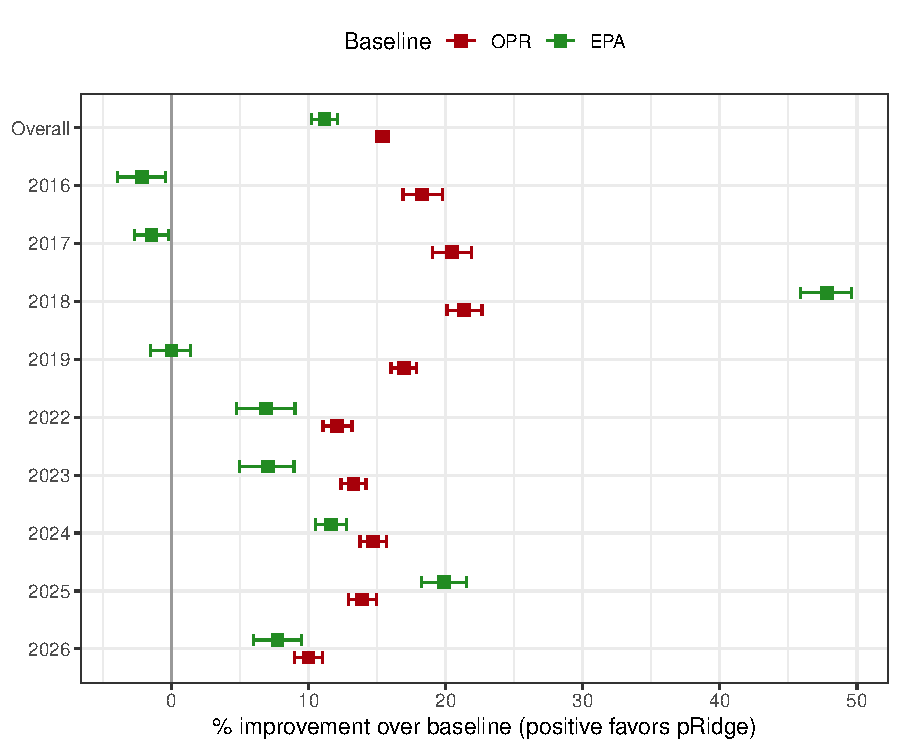
\includegraphics[keepaspectratio]{index_files/figure-pdf/fig-forestplot-1.pdf}}

}

\caption{\label{fig-forestplot}Bootstrap confidence interval forest
plot}

\end{figure}%

\subsection{Comparison against OPR}\label{comparison-against-opr}

In terms of cross validated MSE, pRidge improves on OPR by an average of
15.4\% across all qualifier events between 2016 and 2026. The 95\%
bootstrap confidence intervals are outlined in
Table~\ref{tbl-bootstrap}. The confidence interval for the mean ranges
between 15.0\% and 15.8\%, and no yearwise interval covers 0 or below.
Across all 1389 events in the dataset, pRidge underperformed OPR at only
14 of them, 8 of those events being in 2026.

Plotting percent improvement against year (Figure~\ref{fig-opr-year})
shows some yearly variation, which appears to mostly be driven by the
fit of the OPR model to that year's game. For example, pRidge improves
on OPR the least in 2026, by only 10.0\% on average. The 2026 game
features primarily linear, uncapped scoring and limited game piece
scarcity, which lend themselves very well to OPR's linearity
assumptions. By comparison, pRidge overperforms OPR by the most in 2018,
by 21.3\% on average. The 2018 game relied on time-based scoring and had
a snowball dynamic: alliances that won the scale overwhelmingly won the
match \citep{powerup_blog}, and a scale tipped in your favor was easier
to score on. Neither of those dynamics lend themselves well to OPR's key
assumptions.

There may also be meaningful ``era'' effects. pRidge overperforms OPR
more in pre-pandemic seasons (average 19.2\% improvement over 2016-2019)
than in post-pandemic seasons (12.7\% improvement over 2022-2026.) Team
sustainability challenges through the pandemic, the removal of bag \&
tag, the proliferation of swerve drive, and increasing COTS value all
contribute to major differences in the program between those seasons and
may influence this.

The performance of pRidge compared to an OPR baseline is plotted in
Figure~\ref{fig-opr-week}. Over weeks of the season, pRidge appears to
improve slightly better on average at later events, but it is important
to note the small sample size for week 7 qualifying events - we have
only 18 such events in our dataset.

\subsection{Comparison against EPA}\label{comparison-against-epa}

In terms of next-match-prediction error, pRidge improves on EPA by an
average of 11.1\% across all qualifier events between 2016 and 2026. The
95\% bootstrap confidence interval for the mean ranges between 10.2\%
and 12.1\%. Yearwise confidence intervals for pRidge's mean \%
improvement (Table~\ref{tbl-bootstrap}) cover 0 for 2019, are below 0
for 2016 and 2017, and are above 0 for every other year in the dataset.

pRidge overperforms EPA by the most in 2018 by an average of 47.8\%, far
more so than any other year. Our best explanation for this is that the
snowball dynamics in the 2018 game lent themselves to blowouts that were
well explained by prior information. These blowouts might challenge
rating systems to update well, but regularizing over them could smooth
over the issue. Even discarding 2018, pRidge improves on EPA by an
average of 6.75\% of next-match-prediction error on this dataset.

There may also be ``era'' differences in pRidge's performance compared
to EPA, but they are more gradual than with OPR, and require ignoring
2018. Discarding 2018, pRidge actually underperforms EPA by 1.1\% on
average pre-pandemic, but overperforms EPA by 10.7\% on average
post-pandemic. It's initially unintuitive that regularizing towards EPA
could produce results that underperform EPA, but remember that we're
specifically regularizing towards the \emph{pre-event} EPA. pRidge
underperforming EPA in a particular year implies that the OPR update to
the priors was less informative than the EPA update to the priors.

The performance of pRidge compared to an EPA baseline is plotted in
Figure~\ref{fig-epa-week}. Over the weeks of the season, pRidge appears
mostly steady in comparison to EPA. Again, there are too few week 7
qualifying events (n = 18) to make inferences about the late-season
dynamics.

\section{Discussion}\label{discussion}

Prior Ridge gives a meaningful, reasonably consistent improvement in
team rating on OPR and EPA baselines. Against both baselines, pRidge's
relative performance appeared to change pre- and post-pandemic;
improving against the EPA baseline, and reducing in improvement against
the OPR baseline.

\subsection{Limitations}\label{limitations}

Prior Ridge inherits the limitations of the models it is built on. Like
OPR, it does not model interaction effects. Like EPA, it is biased
towards historical performance. It is not incorporating any new
information, just balancing the bias-variance tradeoff between those two
methods. As with OPR, pRidge summarizes performance in qualification
matches - the alliance interaction dynamics that come out in the
playoffs make modeling playoff performance substantially different.

Another noteworthy limitation: we did not evaluate the performance of
Prior Ridge at the DCMP or CMP level. The differences in play patterns
between qualifier events and higher levels of play may impact difference
in performance between Prior Ridge and other rating systems.

\subsection{Next Steps}\label{next-steps}

There are a few clear avenues to improving on Prior Ridge. For one, the
current model assumes a constant \(\lambda\). However \(\lambda\) could
be a vector with a length equal to the number of competing teams, making
the model more flexible. Optimizing \(\lambda\) as a vector would be
more computationally intensive, but could be a better fit for the data.
This highlights another clear path to improvement for Prior Ridge:
searching the \(\lambda\) grid. Currently we evaluate all candidate
values of \(\lambda\) in the grid, but efficiently searching the
solution space could make the fit much faster.

Experimenting with different priors may improve the model. For example,
for late-season events, once every team has played at least once,
season-max OPR may be a better prior than EPA. Additionally, comparing
pRidge's performance to OPR in a next-match-prediction framework could
give more insight into how well pRidge solves OPR's stabilization
challenges. OPR is typically extremely variable until about 6 matches
per team have been played; pRidge provides an automatic balancing for
this by rolling off \(\lambda\) as more matches are played.

\section{Technical Appendix}\label{technical-appendix}

Code results rely on the
\href{https://github.com/GKrotkov/scoutR}{scoutR} package, available on
GitHub. To install, call \texttt{pak::pak("gkrotkov/scoutR")} in your R
console. The scoutR documentation can be found at
\url{https://gkrotkov.github.io/scoutR/}.

\begin{itemize}
\tightlist
\item
  pRidge testing against OPR
  (\href{https://github.com/GKrotkov/pRidge_eval/blob/main/R/2_pridge_opr_comparison.R}{code})
\item
  pRidge testing against EPA
  (\href{https://github.com/GKrotkov/pRidge_eval/blob/main/R/2_pridge_epa_comparison.R}{code})
\item
  Visualization
  (\href{https://github.com/GKrotkov/pRidge_eval/blob/main/R/3_pridge_viz.R}{code})
\end{itemize}

\subsection{Prior Ridge Coefficient Derivation}\label{sec-derivation}

Define:

\[
\begin{aligned}
\hat{\beta}: \text{prior ridge coefficients}, \quad
\beta_0: \text{priors}, \quad
X: \text{data matrix}, \\
y: \text{response vector}, \quad
L: \text{loss function}, \quad \lambda: \text{regularization penalty}
\end{aligned}
\]

\subsubsection*{Loss Function}\label{loss-function}
\addcontentsline{toc}{subsubsection}{Loss Function}

\[
L(\hat{\beta}) = \| y - X\hat{\beta} \|_2^2 + \lambda \| \hat{\beta} - \beta_0 \|_2^2
\]

By \(L_2\) norm definition:

\[
L(\hat{\beta}) = (y - X\hat{\beta})^{T} (y - X\hat{\beta}) +
\lambda (\hat{\beta} - \beta_0)^{T} (\hat{\beta} - \beta_0)
\]

\subsubsection*{Compute Loss Gradient}\label{compute-loss-gradient}
\addcontentsline{toc}{subsubsection}{Compute Loss Gradient}

\[
\nabla_{\hat{\beta}} L(\hat{\beta})
= \nabla_{\hat{\beta}} [(y - X\hat{\beta})^{T} (y - X\hat{\beta})]
+ \lambda \nabla_{\hat{\beta}} [(\hat{\beta} - \beta_0)^{T} (\hat{\beta} - \beta_0)]
\]

Apply the chain rule and the matrix identity
\(\nabla_{x} (x^{T}A x) = (A + A^{T})x = 2A x\) (for symmetric \(A\)):

\[
\begin{aligned}
\nabla_{\hat{\beta}} L(\hat{\beta})
&= 2(y - X\hat{\beta})\nabla_{\hat{\beta}}[y - X\hat{\beta}] + \lambda * 2(\hat{\beta} - \beta_0) * \nabla_{\hat{\beta}} \hat{\beta} \\
&= -2X^T(y - X\hat{\beta}) + 2\lambda(\hat{\beta} - \beta_0)
\end{aligned}
\]

\subsubsection*{Set Gradient to Zero}\label{set-gradient-to-zero}
\addcontentsline{toc}{subsubsection}{Set Gradient to Zero}

\[
\nabla_{\hat{\beta}} L(\hat{\beta}) = 0
\]

\[
0 = -2X^{T}(y - X\hat{\beta}) + 2\lambda(\hat{\beta} - \beta_0)
\]

Simplify:

\[
\begin{aligned}
- X^{T}y + X^{T}X\hat{\beta} + \lambda \hat{\beta} - \lambda \beta_0 &= 0 \\
X^TX\hat{\beta} + \lambda\hat{\beta} &= X^Ty + \lambda\beta_0 \\
(X^{T}X + \lambda I)\hat{\beta} &= X^{T}y + \lambda \beta_0
\end{aligned}
\]

\[
\boxed{
\hat{\beta} = (X^{T}X + \lambda I)^{-1}(X^{T}y + \lambda \beta_0)
}
\]

\section*{References}\label{references}
\addcontentsline{toc}{section}{References}

\renewcommand{\bibsection}{}
\bibliography{references.bib}





\end{document}
